% !TEX encoding = UTF-8 Unicode
% -*- coding: UTF-8; -*-
% vim: set fenc=utf-8
\documentclass[a4paper,12pt,french]{article}

\usepackage{centrale}

\hypersetup{
  pdftitle={Compte-Rendu TP3},
  pdfauthor={Aymeric ZIMINSKI / Zaryus},
  pdfsubject={Compte-rendu TP3},
  pdfproducer={Conversion PDF},
  pdfkeywords={Quelques mots-clés} %
}

\DeclareGraphicsRule{.ai}{pdf}{.ai}{} % Pour insérer des documents .ai
\graphicspath{{./img/} {./eps/} {./fig/}} % Pour ne pas avoir à ajouter eps/ton-image.jpg

% ------------- Packages spéciaux, nécessaires pour ce rapport, à insérer ici ------------- 
\usepackage{minted}


\begin{document}

% --------------------------------------------------------------
%                       Page de garde
% --------------------------------------------------------------

\begin{titlepage}
  \begin{center}

    
\includegraphics[width=0.5\textwidth]{LogoECN.jpg}\\[1cm]

    {\large Electronique}\\[0.5cm]
    {\large Systèmes Embarqués Communiquants}\\[0.5cm]

    % Titre
    \rule{\linewidth}{0.5mm} \\[0.4cm]
    { \huge \bfseries TP3 : Étude d'une alimentation buck\\[0.4cm] }
    \rule{\linewidth}{0.5mm} \\[1.5cm]

    % Auteur(es) et encadrant(es)
    \noindent
    \begin{minipage}{0.4\textwidth}
      \begin{flushleft} \large
        \emph{Auteur :}\\
        M. Guillaume \textsc{PIRAUBE}\\
        M. Aymeric \textsc{ZIMINSKI}
      \end{flushleft}
    \end{minipage}%
    \begin{minipage}{0.4\textwidth}
%      \begin{flushright} \large
%        \emph{Encadrants :} \\
%        M.~Prénom \textsc{Nom}\\
%        M.~Prénom \textsc{Nom}
%      \end{flushright}
    \end{minipage}

    \vfill

    % Date en fin de page
    {\large Version du\\ \today}

  \end{center}
\end{titlepage}

% --------------------------------------------------------------
%                    Table des matières 
% --------------------------------------------------------------

\thispagestyle{empty}
\tableofcontents
\pagebreak

% --------------------------------------------------------------
%                         Début du corps
% --------------------------------------------------------------

\section{Introduction}

L'objectif de ce TP est de réaliser une étude sur une alimentation à découpage de type buck. Nous allons utiliser le composant MC34063 de Microchip.

Nous devrons mettre en application la théorie que nous avons vu en cours, notamment sur alimentations à découpage et leurs caractéristiques.


% --------------------------------------------------------------
%                         Partie 1
% --------------------------------------------------------------

\pagebreak
\section{Commande en boucle ouverte}
\subsection{Commande de la PWM à 100kHz}

Nous souhaitons dans un premier temps connaître le rapport cyclique nécessaire pour que le buck soit en mode CCM.

Nous savons que en CCM, le rapport cyclique est égal à $\frac{V_{out}}{V_{in}}$. Nous avons que $V_{out} = 3.3 V$ et $V_{in} = 10 V$, donc :

\[
  \alpha = \frac{V_{out}}{V_{in}} = \frac{3.3}{10} = 0.33
\]

En mode DCM, avec un rapport tension de 0.33, nous avons un rapport cyclique inférieur à celui du mode CCM, donc $\alpha < 0.33$.

\begin{figure}[H]
    \centering
    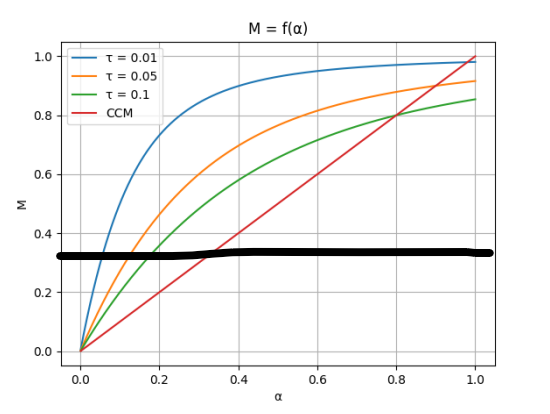
\includegraphics[width=0.6\textwidth]{graphique_alpha.png}
    \caption{Rapport de tension en fonction du rapport cyclique}
    \label{fig:graphique1}
\end{figure}

\vspace{1cm}

Nous souhaitons maintenant implémenter une PWM de 100KHz.

\begin{minted}{c}
  void setupTIM_PWM2()
  {
    RCC->APB1ENR |= RCC_APB1ENR_TIM2EN;
    __asm("nop");
    //reset peripheral (mandatory!)
    RCC->APB1RSTR |= RCC_APB1RSTR_TIM2RST;
    RCC->APB1RSTR &= ~RCC_APB1RSTR_TIM2RST;
    __asm("nop");


    //config timer2@100KHz, with 10 ticks
    TIM2->PSC = 1-1; //prescaler : tick@1us
    TIM2->ARR = 2400-1; //auto-reload: counts 10 ticks → 10µs → 100KHz
  
    PWMEnableChannel(TIM2, 2);
    TIM2->CCR2 = (TIM2->ARR)/3-1;
    TIM2->CR1 |= TIM_CR1_CEN;
  }

\end{minted}

Après vérification de la tension au bornes du pin de la PWM, nous avons bien une PWM de fréquence 100 kHz. Ce qui est conforme aux spécifications demandées.

\vspace{1cm}

Après vérification du montage, nous avons brancher la PWM sur l'entré de la buck. Nous regardons la tension auprès de la diode. 

Après avoir augmenter la fréquence, nous observons la résonnance du condensateur (figure \ref{fig:q4}). 

\begin{figure}[H]
    \centering
    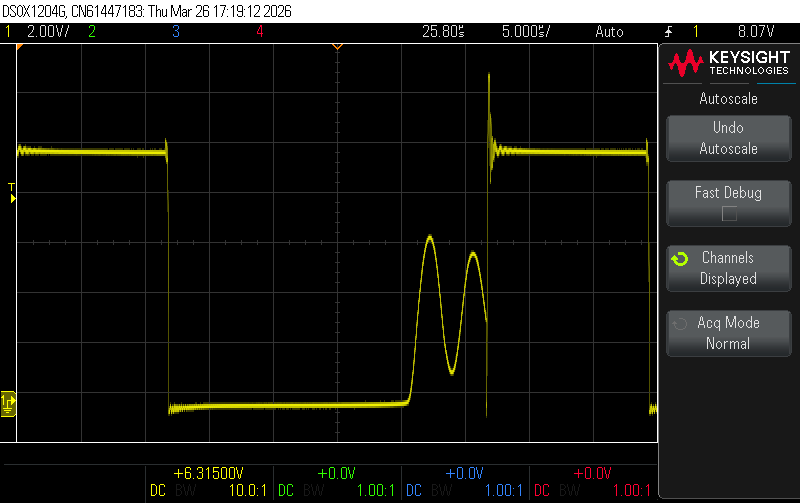
\includegraphics[width=0.6\textwidth]{Q4.png}
    \caption{Sortie de la buck}
    \label{fig:q4}
\end{figure}

Nous observons que la tension de la buck commence à avoir cette résonnance à partir de 40 kHz. 

\subsection{Lecture de la tension de sortie}

Nous souhaitons lire la tension de sortie du buck. Pour se faire, nous avons à notre disposition la broche PA3 de la nucléo qui est un ADC sur 12 bits.

Nous allons alors réaliser la lecture de $V_out$ et nous allons envoyer cette valeur sur la ligne série en mV. On pourra ensuite valider notre résultat en la comparant avec notre observation à l'oscilloscope.

Nous avons alors modifié la fonction setup de notre projet de la manière suivante :
\begin{minted}{c}
void setup() {
  ADCInit();
  setupTIM6();
  RCC->AHBENR |= RCC_AHBENR_GPIOBEN;
  pinMode(GPIOB,4,OUTPUT); //PB4 => D12
  pinAlt(GPIOB, 3, 1);
}
\end{minted}

En rajoutant ADCInit(), cela permet d'initialiser notre ADC. Nous avons ensuite réalisé la fonction float readVout() suivante :
\begin{minted}{c}
float readVout(){
  Serial.printInt(ADCRead());
  Serial.printchar('\n');
  return ADCRead();  
}
\end{minted}

Nous avons fais en sorte que la fonction readVout() soit appelée dans la fonction d'intérruption du timer 6 :
\begin{minted}{c}
  extern "C" void TIM6_DAC1_IRQHandler()
{
  readVout();
  TIM6->SR &= ~TIM_SR_UIF; //ack
}
\end{minted}

Ainsi nous avons pu observer les messages suivant sur la liaison série (figure \ref{fig:Q5_liaison_série}).
\begin{figure}[H]
    \centering
    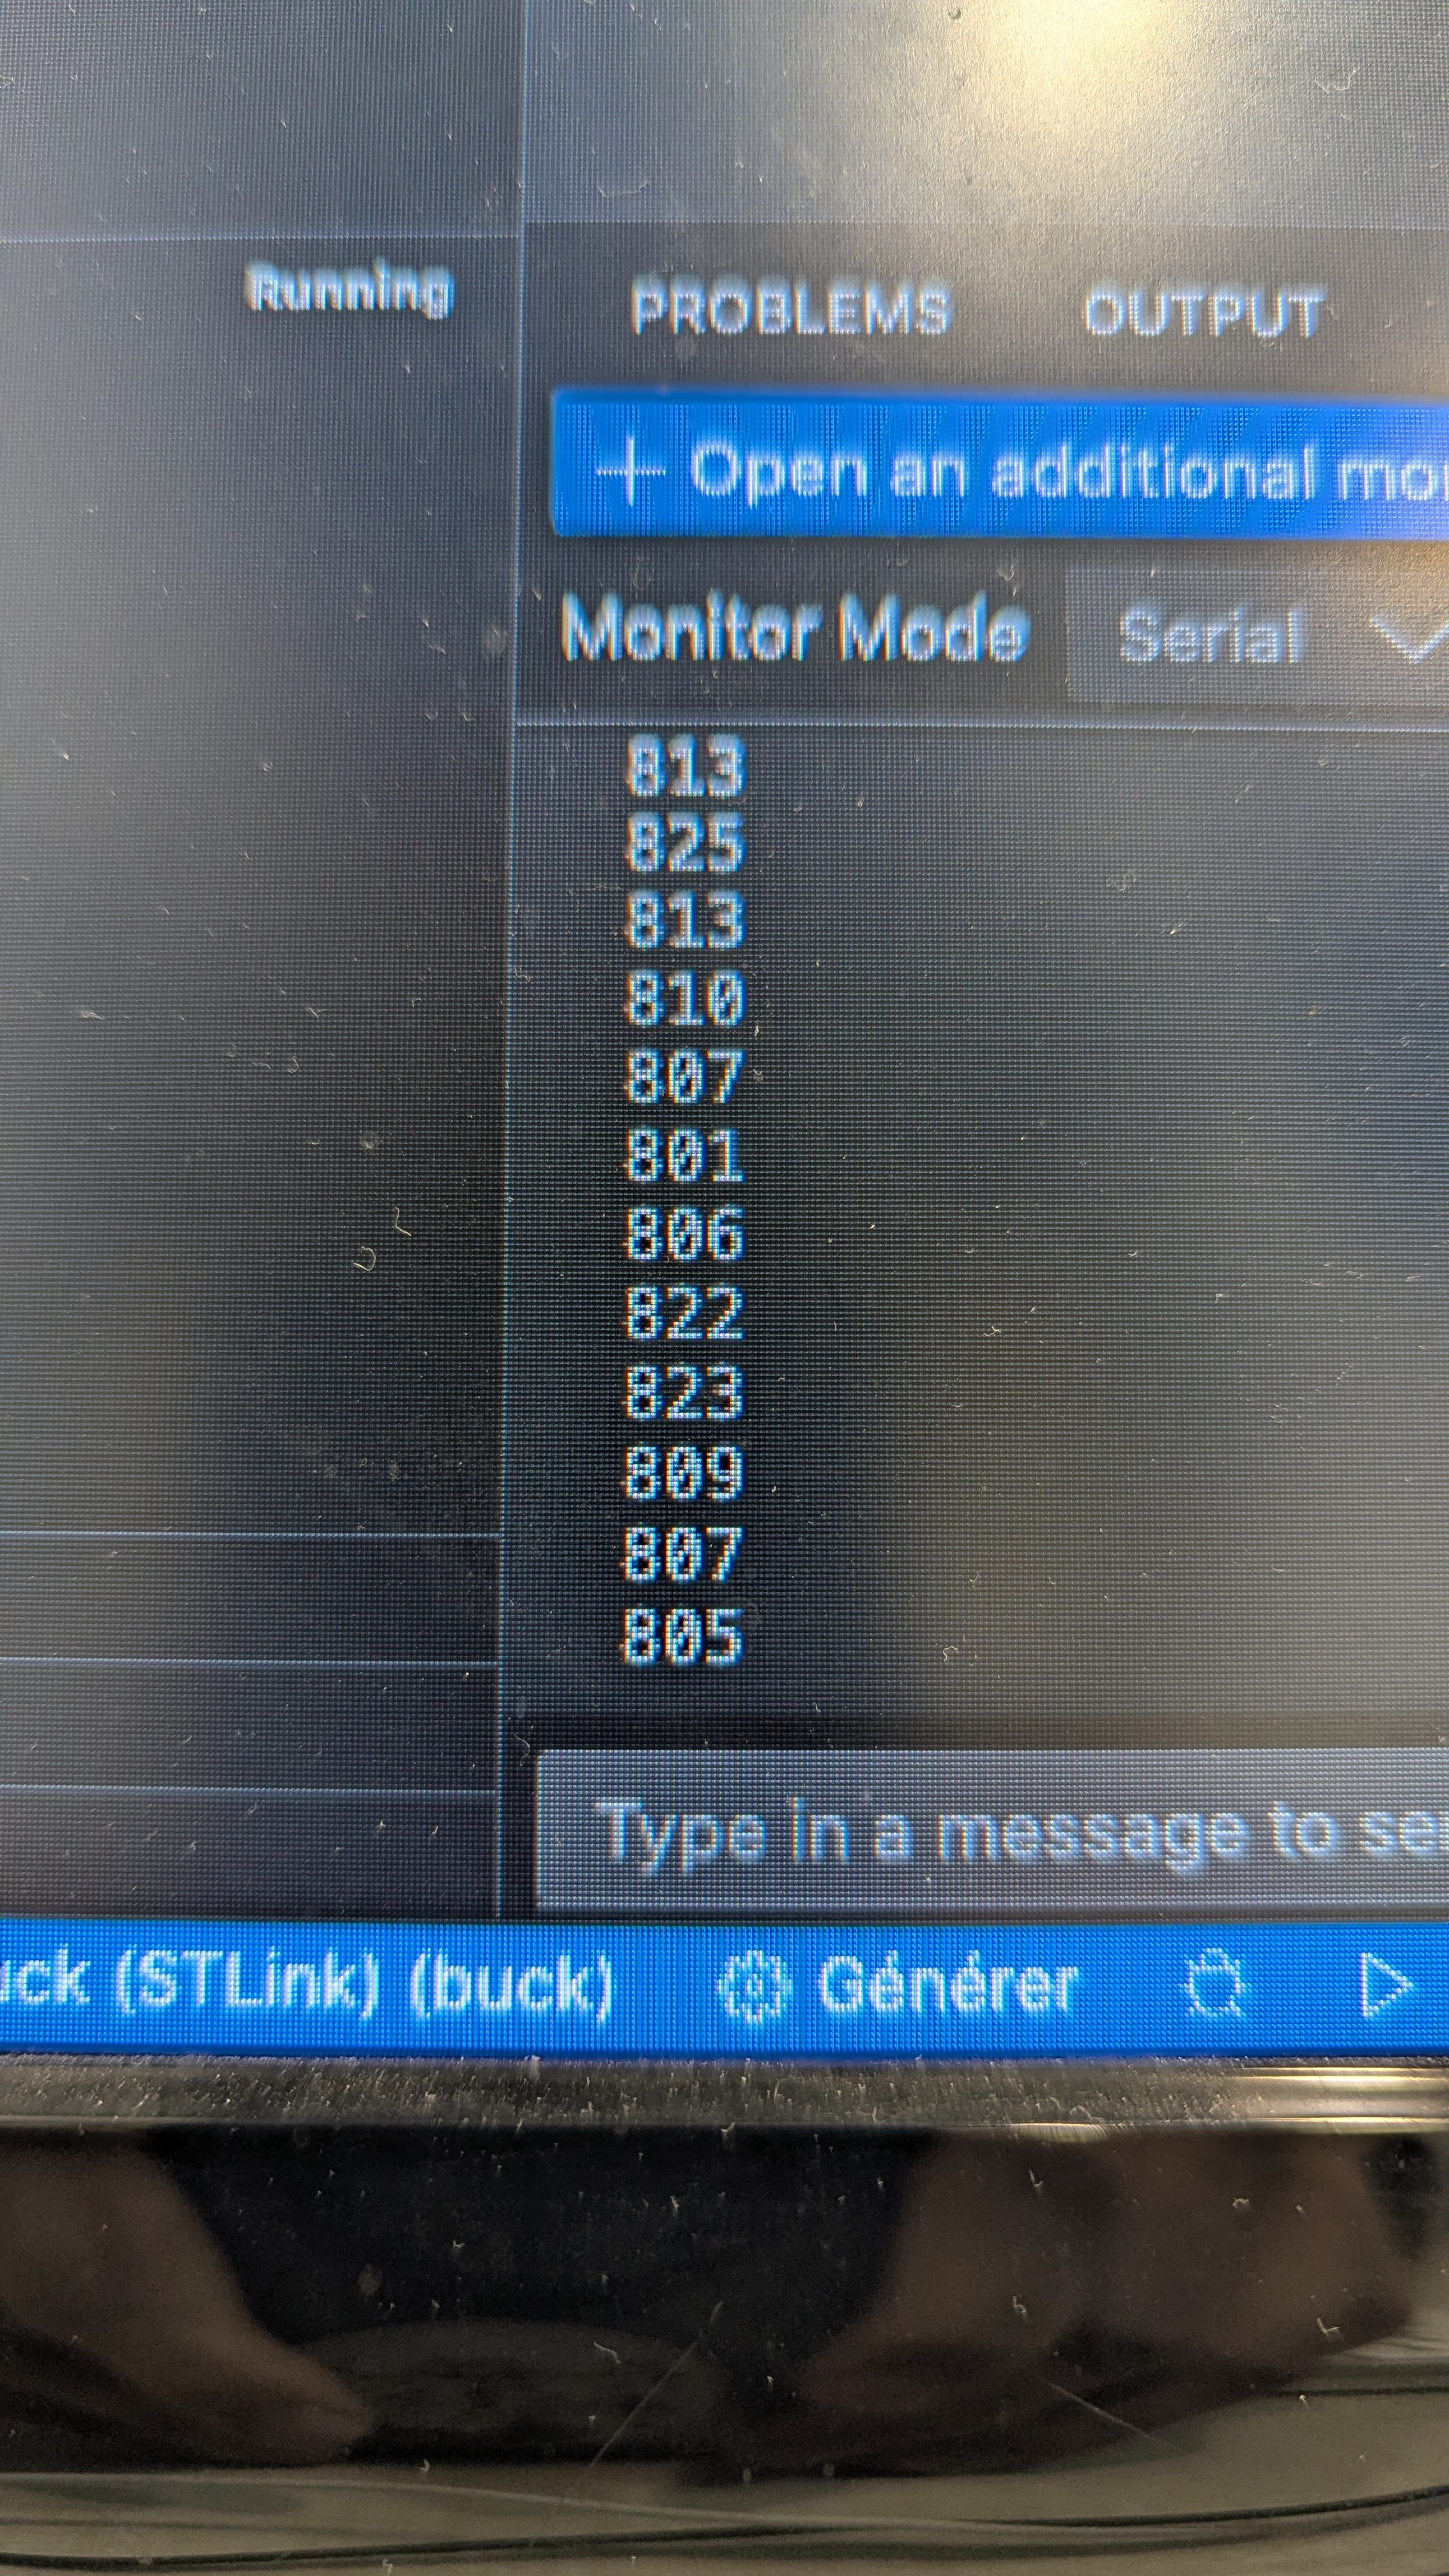
\includegraphics[width=0.6\textwidth]{Q5_1.jpg}
    \caption{Communication série de la fonction readVout()}
    \label{fig:Q5_liaison_série}
\end{figure}

Et nous avons pu confirmer le bon fonctionnement en observant la tension sur l'oscilloscope (figure \ref{fig:Q5_oscillo}).
\begin{figure}[H]
    \centering
    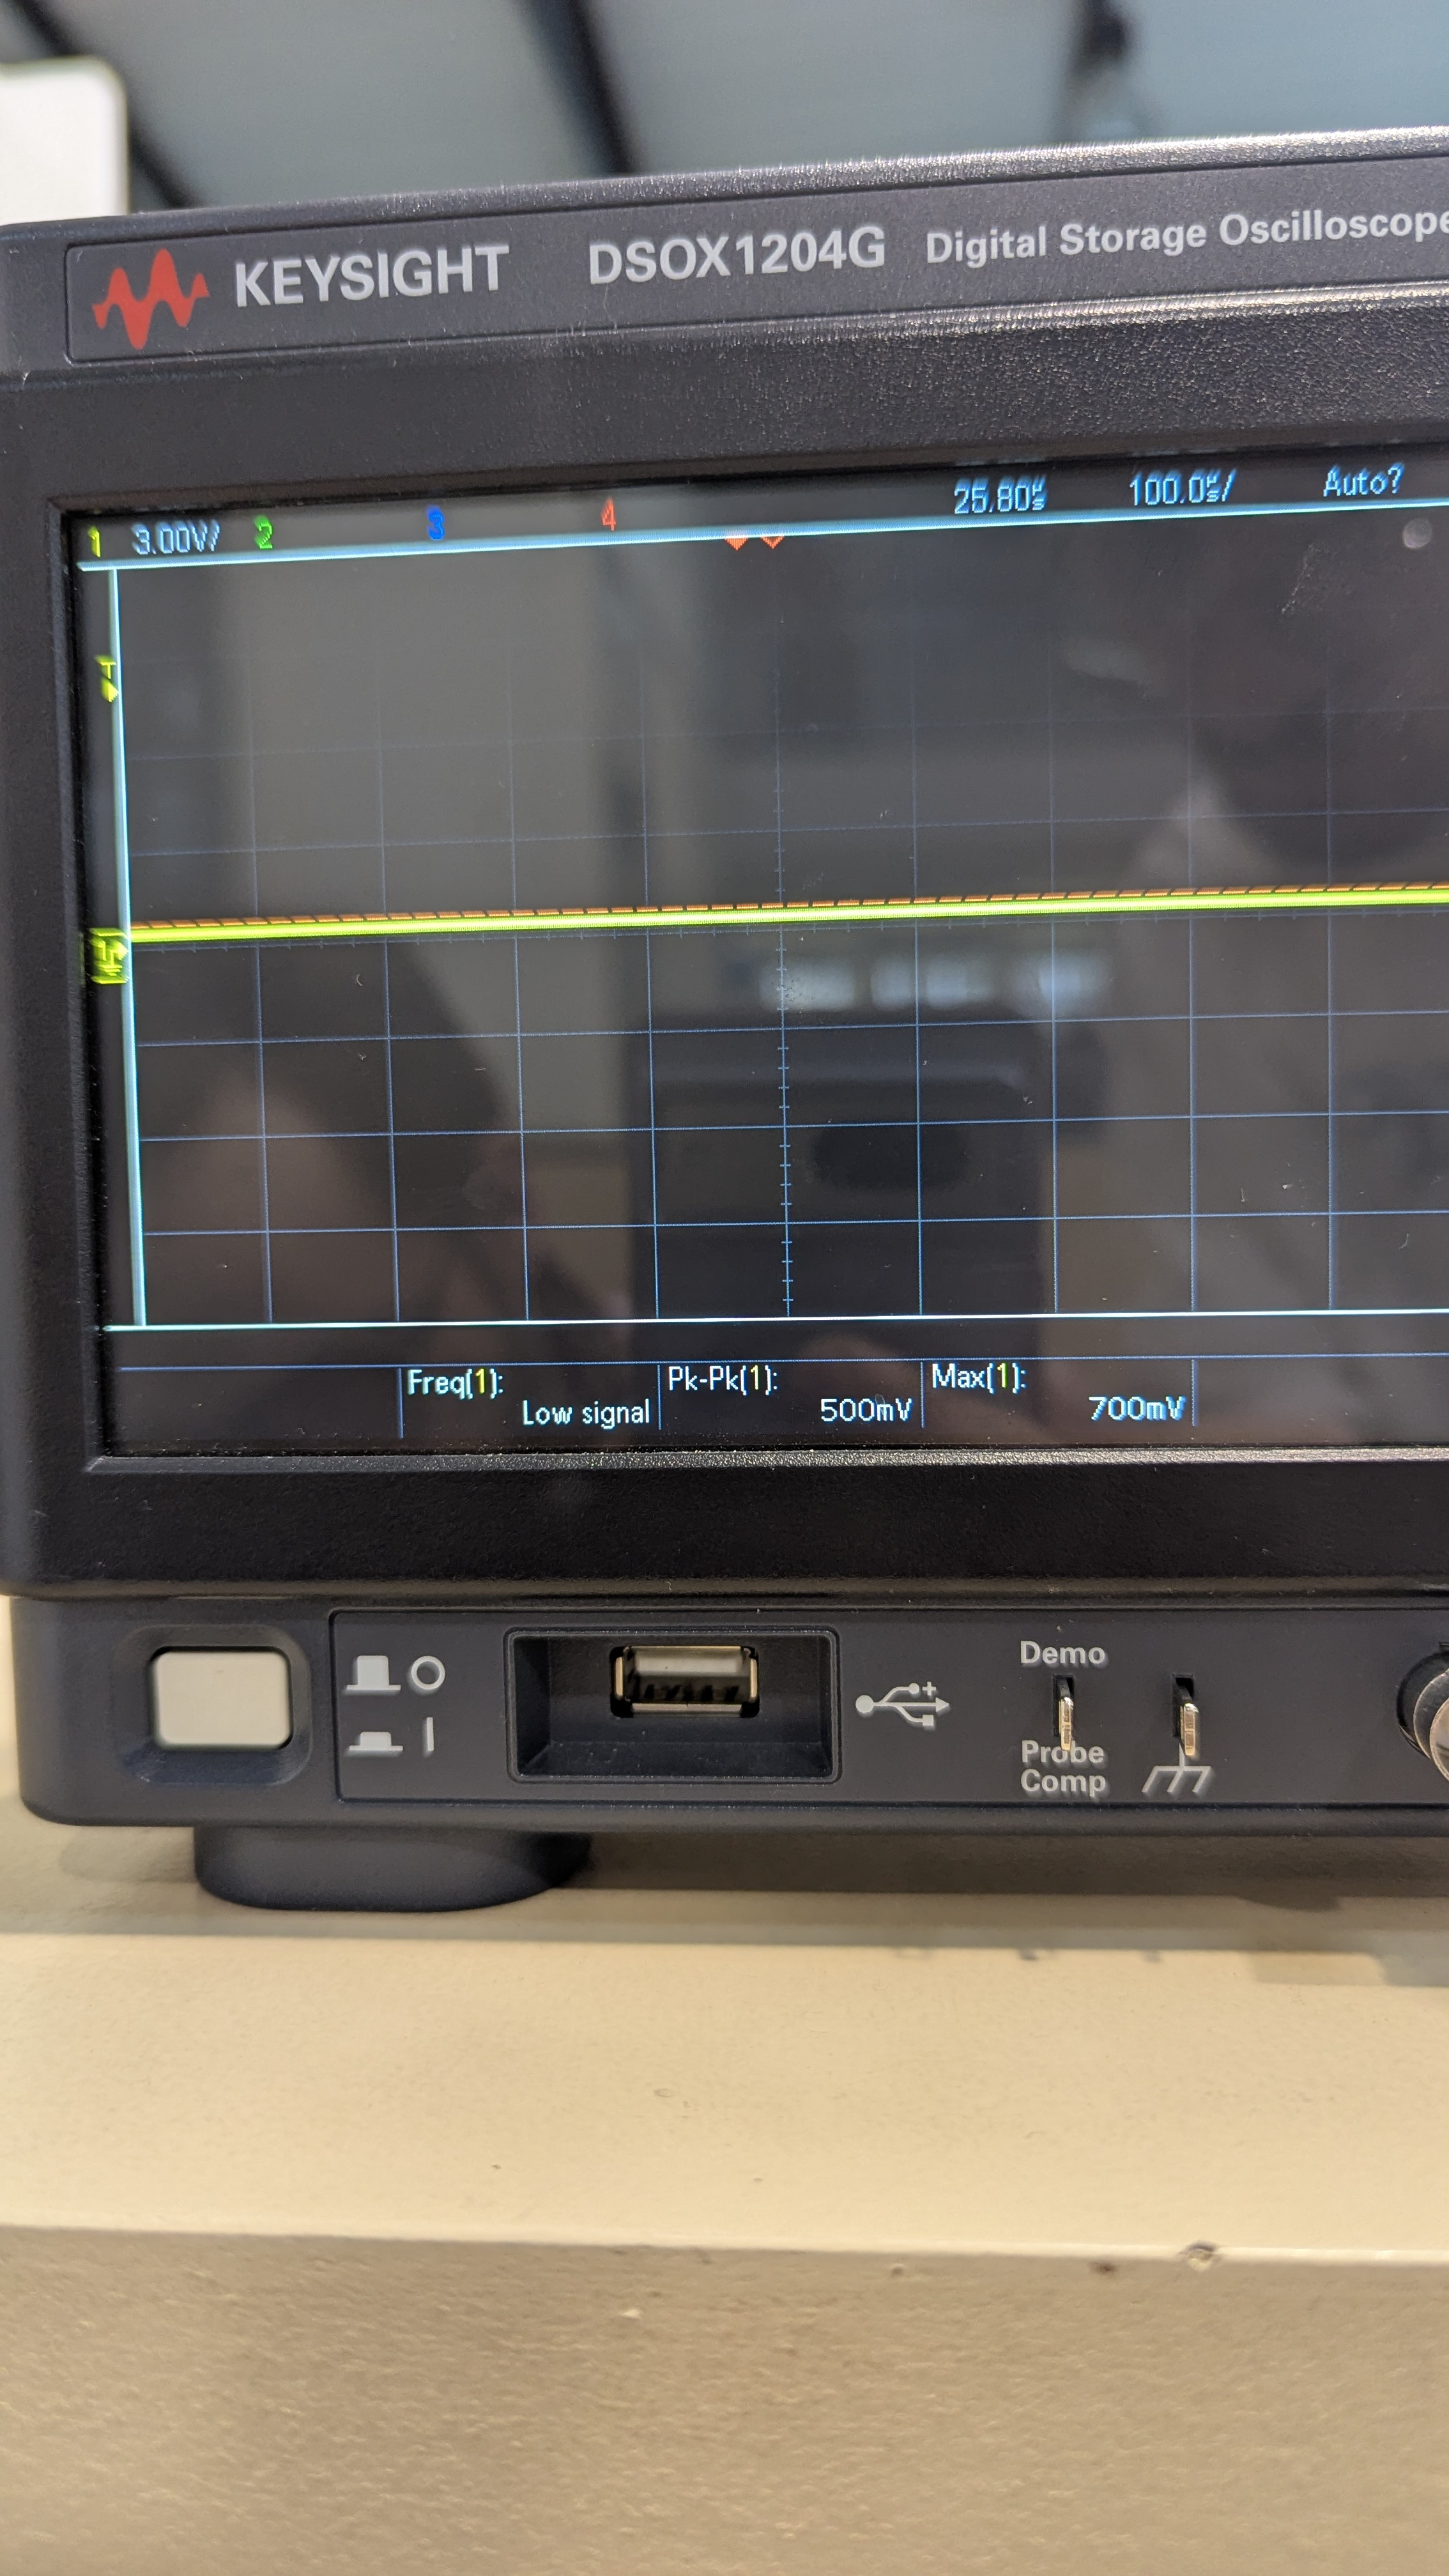
\includegraphics[width=0.6\textwidth]{Q5_2.jpg}
    \caption{Observation de la tension de sortie pour valider la fonction readVout()}
    \label{fig:Q5_oscillo}
\end{figure}

Nous avons relever une différence de 100mV entre la mesure de l'oscilloscope et de la liaison série.

Nous souhaitons maintenant connaître le temps d'acquisition de l'ADC. Pour se faire, nous allons utiliser la broche PB4 que nous allons toggle avant et après chaque mesure.

Nous avons donc modifié le code de la fonction float readVout() de la manière suivante :
\begin{minted}{c}
float readVout(){
  digitalToggle(GPIOB,4);
  Serial.printInt(ADCRead());
  digitalToggle(GPIOB,4);
  Serial.printchar('\n');
  return ADCRead();  
}
\end{minted}

La broche PB4 s'active et se désactive entre chaque mesure de l'ADC. Nous avons alors observé à l'oscilloscope le signal suivant sur la broche PB4 (figure \ref{fig:Q6_oscillo}).

\begin{figure}[H]
    \centering
    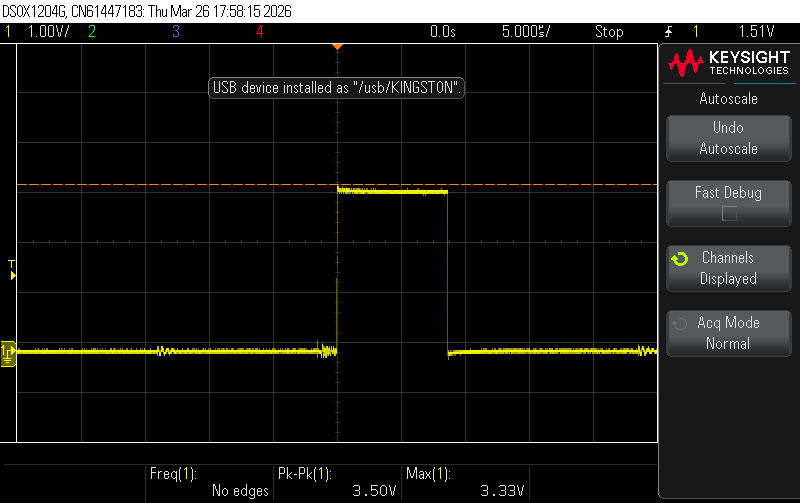
\includegraphics[width=0.6\textwidth]{Q6.png}
    \caption{Observation du signal de la broche PB4}
    \label{fig:Q6_oscillo}
\end{figure}

Nous avons pu relever le temps entre chaque acquisition qui est de 8µs.

\pagebreak
\subsection{Limites en boucle ouverte}

Nous souhaitons maintenant observer la tension de sortie en fonction de la charge. Nous allons donc changer la valeur de la résistance de charge.

Nous avons observer les signaux suivants (figure \ref{fig:Q7_oscillo_1} et figure \ref{fig:Q7_oscillo_2}).
\begin{figure}[H]
    \centering
    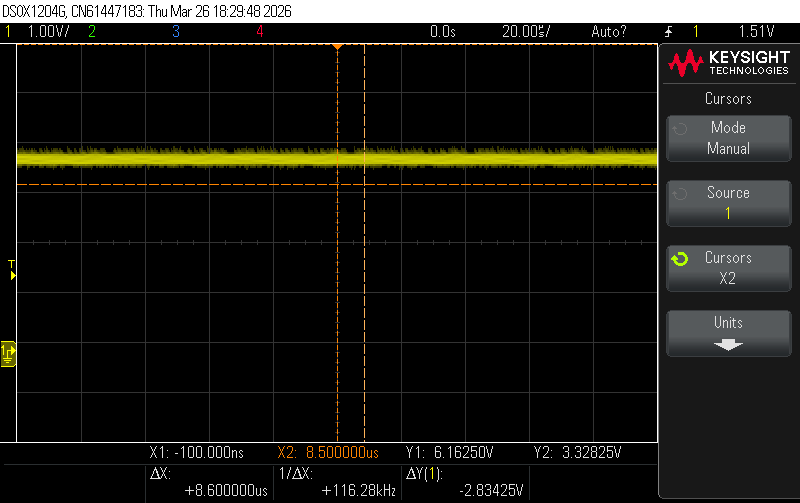
\includegraphics[width=0.6\textwidth]{Q7_1.png}
    \caption{Observation du signal de sortie avec la première charge}
    \label{fig:Q7_oscillo_1}
\end{figure}

\begin{figure}[H]
    \centering
    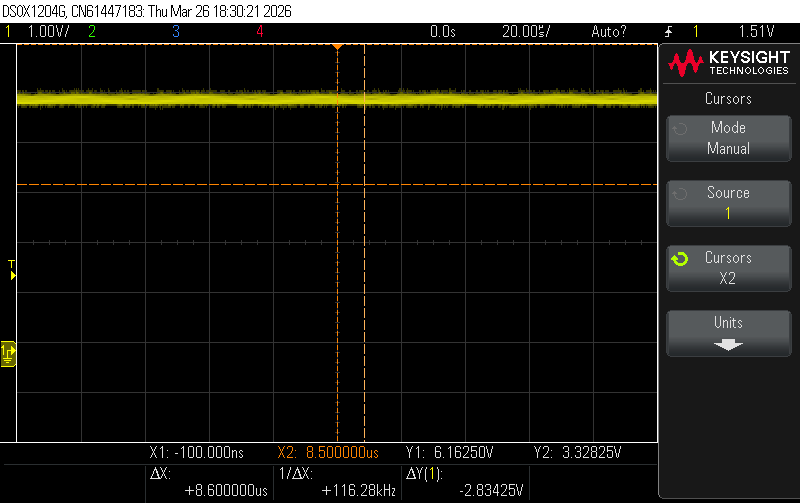
\includegraphics[width=0.6\textwidth]{Q7_2.png}
    \caption{Observation du signal de sortie avec la seconde charge}
    \label{fig:Q7_oscillo_2}
\end{figure}

Nous pouvons voir que la tension de sortie varie en fonction de la charge qui est au borne de l'alimentation à découpage. Cela est dû au rapport cyclique qui est fixe. Pour éviter que la tension de sortie varie en fonction de la charge, il faudrait faire en sorte de le recalculer en récupérant la valeur de sortie avec l'ADC et trouver ensuite une relation entre le rapport cyclique et la tension de sortie.

% --------------------------------------------------------------
%                            Conclusion
% --------------------------------------------------------------

\pagebreak
\section{Conclusion}

Nous n'avons pas eu le temps de traiter l'ensemble des questions du TP mais nous avons pu appliquer les notions vu en cours sur l'alimentation à découpage. Nous avons pu la caractériser en boucle ouverte et voir les limites qui étaient présente nottament à la fin avec la tension de sortie qui varie en fonction de la charge qui est au borne de l'alimentation.\\

% --- Biblio par .bib
%\bibliography{ici-ton-fichier-biblio}
%\bibliographystyle{plain-fr.bst}
%\selectlanguage{french}

% --- Biblio écrite à la main
%\begin{thebibliography}{7}
%\bibitem[Bastien 2019]{id-de-la-source}
%Auteurs : \emph{Un titre},  une date.
%\end{thebibliography}

% --------------------------------------------------------------
%                            Appendices
% --------------------------------------------------------------

%\pagebreak
%\appendix
%\begin{appendices}
%\section{}


%\end{appendices}

\end{document}
